\documentclass{article}
\usepackage[margin=1in]{geometry}

\usepackage{fancyvrb}
\usepackage[skins, raster, minted]{tcolorbox}
\usepackage{minted}
\usepackage{varwidth}
\usepackage{multicol}
\usepackage{bytefield}
\usepackage[colorlinks=true]{hyperref}
\usepackage{graphicx}

\newtcolorbox{info}[1]{colbacktitle=blue!20!white, coltitle=black, title={#1}}
\newtcblisting{gas}[1]{listing engine=minted, minted language=gas, minted style=colorful, listing only, title={#1}}
\newtcblisting{ld}[1]{listing engine=minted, minted language=text, minted style=colorful, listing only, title={#1}}

\graphicspath{{figures/}}

\title{OS From Scratch \\ \large Why? Because why not.}
\author{James Geiss}
\date{October 2023}

\begin{document}
\maketitle
\newpage

{
	\hypersetup{linkcolor=black}
	\tableofcontents
	\newpage
}

\section{Purpose}

This document will likely never reach anyone, but I thought that collecting my thoughts and cataloging
my understanding and design choices along my journey building an operating system would be an effective
means of education for myself, and anyone who may see this.

What was the actual reason for embarking on this project? As I mentioned before, I do not have one.
I simply wanted to learn more about the workhorses that keep the world running on top of what is, in
essense, a pile of finely tuned metal.

If your at any length curious, come along for as long as you like. Or until I get bored and move onto
something more rewarding than reinventing something argueably more commonplace than a wheel.

\newpage

\section{Boot}

\subsection{UEFI}
The boot process of most modern computers is started with the Unified Extensible Firmware Interface (UEFI),
which is reponsible for handing over your kernel the reigns after setting up a nice and polished workspace for
you to connect up to.

\subsection{BIOS}
Forget UEFI, that takes the fun out of it. Why boot straight to the kernel with a few lines of C when you can
do it from scratch; that is the point of this, is it not? We are going to cut back down to the BIOS, the
``Basic Input/Output System'', who's sole purpose is to give you the bare minimum needed to start an operating
system.

All the BIOS does is provide some helpful backend functions (interrupts) that let us do some basic standardized
communication with the underlying hardware and just launches the bootsector, plain and simple. The
bootsector is simply sector one of the boot drive, where a ``sector'' is 512 bytes of data starting
with sector one. The only requirement is that the last two bytes of the sector are \Verb{0xAA55}.

Technically, this is a valid, bootable system image:

\begin{figure}[H]
	\LVerbatimInput{figures/empty_bootsector.txt}
	\label{fig:empty_bootsector}
\end{figure}

\begin{info}{Endianness}
	Why are the last two bytes \Verb{0x55AA} and not \Verb{0xAA55}? That's endianness.
	Endianness describes the order of bytes in a value when placed into a memory address.
	There are two endianesses: little and big. Let's look at the value \Verb{0xABCDEF}:
	
	\begin{multicols}{2}
		\textbf{Little Endian}
		In little endian, the \emph{Least Significant Byte} (LSB), comes first.
		
		\columnbreak
		
		\textbf{Big Endian}
		In big endian, the \emph{Most Significant Byte} (MSB), is placed first.
	\end{multicols}
	
	\begin{multicols}{2}
		\begin{center}
			\begin{bytefield}[bitwidth=0.1\linewidth]{3}
				\bitheader[endianness=big]{2, 1, 0} \\
				\bitboxes{1}{{EF} {CD} {AB}}
			\end{bytefield}
		\end{center}
		
		\columnbreak
		
		\begin{center}
			\begin{bytefield}[bitwidth=0.1\linewidth]{3}
				\bitheader[endianness=big]{2, 1, 0} \\
				\bitboxes{1}{{AB} {CD} {EF}}
			\end{bytefield}
		\end{center}
	\end{multicols}
	
	Notice that the bits are \textbf{not} reversed.
\end{info}

\subsection{Barebones}

It should be pretty obvious by now that with only 512 bytes of space available to us, we won't be booting into
a fancy low-level language like C. That's right, x86 assembly it is.

First things first, pick an assembler. At the time of righting, the nicest one is probably \emph{NASM}; however,
since we will be making extensive use of the \emph{GNU} famply of tools, the rest of of this document will be
tailored for the \emph{GNU Assembler} (GAS), though the instructions will be (nearly) indenticle.

Let's start off first by filling in those empty spaces up to the last two bytes and writing in our magic
bootsector number. There will be a fancier solution for this down the line, but let's start here:

\begin{gas}{bootsector.s}
	.intel_syntax noprefix
	.code16
	
	_start:
		jmp .
	
	.space 510 - (. - _start)
	.word 0xaa55
\end{gas}

The line \mintinline{gas}|.space 510 - (. - _start)| fills the number of bytes needed between the current
location in the file (\Verb|.|) and the start of the file (\Verb|_start|) up to 510 bytes. Remember, we need to
leave in the last two bytes to fill in our magic number, which we can add with \mintinline{gas}|.word 0xaa55|.
The instruction \mintinline{gas}|jmp .| jumps to the current address (an infinite loop).

We will also need to make sure to add the \Verb|.code16| directive, to make sure that GAS compiles 16-bit assembly.
Why? Because unfortunately for us, the BIOS drops us off not in 64-bit mode, not in 32-bit mode, and not even
in \emph{Protected Mode}. Our bootsector is run in 16-bit \emph{Real Mode}.

\begin{info}{Syntax}
	There are two major assembly syntax styles: AT\&T and Intel.
	
	\begin{multicols}{2}
		\textbf{AT\&T}
		
		\mintinline{gas}|movl $10, %eax|
		
		\columnbreak
		
		\textbf{Intel}
		
		\mintinline{gas}|mov eax, 10|
	\end{multicols}
	
	I know which one I'm going to use.
\end{info}

We can compile this assembly file with the command:

\begin{Verbatim}
	as -o bootsector.o bootsector.s
\end{Verbatim}

Make sure to have installed GAS using your system's package management solution. This will output an \emph{Executable and Linkable Format} (ELF) file. To get it into a binary, we need to use the linker:

\begin{Verbatim}
	ld --oformat binary -o bootsector.bin bootsector.o
\end{Verbatim}

This will output a file similar the one above (\ref{fig:empty_bootsector}).

\subsection{Emulation}

Great. Now... how do we test it? This is where emulation comes in. We could use a virtualization solution, but
realistically there is not a reason to setup a full virtual machine at the moment. The best emulation solution
available at the time of writing is \emph{QEMU}, so go ahead and grab that using your installation method of
choice. Then we can run out makeshift bootsector by pretending that it is a hard drive image:

\begin{Verbatim}
	qemu-system-i386 -hda bootsector.s
\end{Verbatim}

If all goes well, you will end up with a screen something like this:

\begin{figure}[H]
	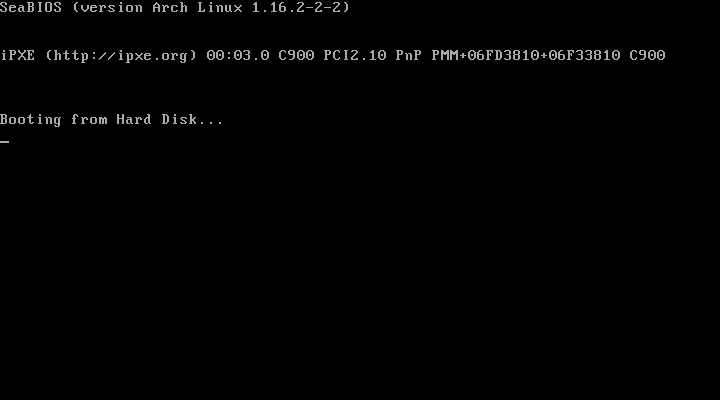
\includegraphics[width=\textwidth]{empty_bootsector.png}
\end{figure}

\subsection{Hello X}

Let's try printing out some text. So... how do we do that? We will use one of those interrupts mentioned
earlier. Specifically, \href{https://en.wikipedia.org/wiki/INT_10H}{interrupt \Verb|10h|}. If we take a look at
the options in that table, we will see a pretty useful one, ``Teletype output ''. In order
to make that happen, we need to:

\begin{enumerate}
	\item Set \Verb|ah| to \Verb|0x0e|
	\item Set \Verb|al| to our character of choice (in ASCII)
	\item Call interrupt \Verb|0x10|
\end{enumerate}

Let's take a look at that in assembly:

\begin{gas}{}
	mov ah, 0x0e
	mov al, 0x58 # The ASCII code for 'X'
	int 0x10
\end{gas}

And if we compile and run, we can see our X printed onto the screen:

\begin{figure}[H]
	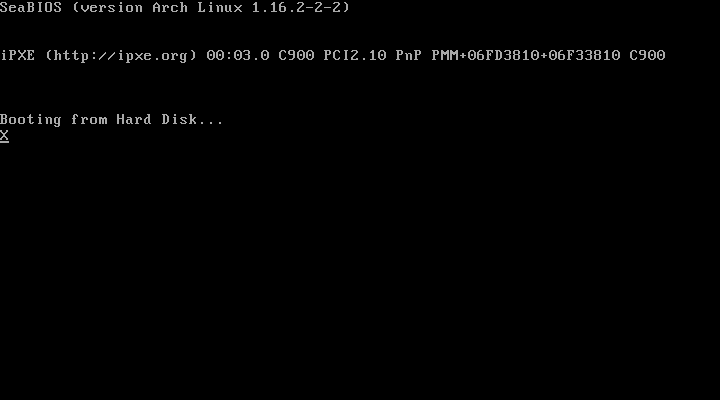
\includegraphics[width=\textwidth]{hellox.png}
\end{figure}

If you want to clear the screen, you will need to reset the video mode (there is no built-in clear operation):

\begin{gas}{}
	mov ah, 0x00 # Set video mode
	mov al, 0x03 # Colored 80x25 text mode
	int 0x10
\end{gas}

\subsection{Memory}

Now, let's try to setup a print string function, instead of just single characters. Although the time we will
be spending in the bootsector is going to be pretty minimal, it's always a good idea to have as much logging
available as possible. If we want to print out a string, we will simply need to print one character at a time
while iterating through a string in memory. But first, we have a problem. Where are we in memory? Although
the bootsector itself exists in sector 1, that is not where it ends up in memory once it is loaded.

The bootsector will get loaded into address \Verb|0x7c00| in memory. If we store a string at the end of the
bootsector try to iterate over it, we will first need to offset it's address by adding \Verb|0x7c00|.
Thankfully, we don't need to do this manually. There are two solutions to this problem. The first is to use
segmentation. Segmentation involves using two registers instead of one when addressing memory, which
artificially expands the addressable memory space in lower addressing modes. Say we wanted to grab the byte
at address 0x0a0001, which is outside of our 16-bit addressable memory space. We could set the data segment
register, \Verb|ds|, to \Verb|0x0a|, and address the lower 2 bytes of our address:
\mintinline{gas}|mov ax, [0x0001]|. This instruction would then implicitly use the \Verb|ds| segment register,
resulting in the effective address:

\begin{center}
	\begin{bytefield}[bitwidth=0.02\linewidth]{32}
		\bitheader[endianness=big]{31, 16, 15, 0} \\
		\begin{rightwordgroup}{0x000A0001}
			\bitboxes{16}{{000A} {0001}}
		\end{rightwordgroup} \\
		\bitboxes{16}{{ds} {ax}}
	\end{bytefield}
\end{center}

The second solution is to use a linker script. A linker script is a GNU specific config file that describes how
we want our output to behave logically. We then feed our linker script to the linker with the \Verb|-T| flag.
Because we will make extensive use of linker scripts for other parts of the compilation process, we will be using
this method; however, we still need to set the segment registers, as their default values vary from system to system.

\subsection{Linking}

We'll start out with a basic linker script:

\begin{ld}{image.ld}
	OUTPUT_FORMAT(binary)
	
	SECTIONS {
		. = 0x7c00;
		
		.text : {
			*(.text)
		}
	}
\end{ld}

The \Verb|.| symbol represents the current location in memory. By setting \Verb|.| to \Verb|0x7c00|, we force
the linker to resolve anything afterwards relative to a \Verb|0x7c00| offset. Then we include the \Verb|.text|
section (the code section) with the rather odd syntax \mintinline{text}|*(.text)|. The prior \Verb|.text| label
does not need to be called \Verb|.text|, and you could use something like \Verb|.boot|.

While we are here, we can also use the linker script to modify the output directly, such as adding our magic
number:

\begin{ld}{image.ld}
	OUTPUT_FORMAT(binary)
	
	SECTIONS {
		. = 0x7c00;
		
		.text : {
			*(.text)
			
			FILL(0x00);
			. = 0x1fe;
			SHORT(0xaa55);
		}
	}
\end{ld}

Within a section, the \Verb|.| symbol is relative, so we can allocate a new word at \Verb|0x1fe| while filling
the empty space with zeros. With this addition, we can remove the \mintinline{gas}|.space| and
\mintinline{gas}|.word| directives from our bootsector, and also drop the \Verb|_start| label.

Next, we need to set the segment registers at the start of our bootsector. For our use case, we will just set
them all to \Verb|0|.

\begin{gas}{bootsector.s}
	xor ax, ax # Functionally equivalent to `mov ax, 0`
	mov ds, ax # Data
	mov es, ax # Extra
\end{gas}

\begin{info}{Immediates}
	We are we loading \Verb|ax| first, instead of just moving in \Verb|0|? Segment registers cannot be set
	directly with an immediate value, a literal, like most registers. Therefore, we first need to set an
	intermediary register, \Verb|ax|, first.
\end{info}

Additionally, there is also a stack segment register \Verb|ss|. Although we do not need it yet, we can set it
while we are here. Unlike the other two, we need to immediately set \Verb|sp| after changing \Verb|ss| in the
next instructions, otherwise our stack will be invalid. We can set it to \Verb|0x7c00| since the stack will
grow downwards and there is free space under our bootloader. This will be updated later anyways.

\begin{gas}{bootsector.s}
	xor ax, ax
	mov ds, ax
	mov es, ax
	mov ss, ax
	mov sp, 0x7c00
\end{gas}

We also need to be absolutely sure than nothing is called inbetween setting \Verb|ss| and \Verb|sp|. Although
we are very low level, in theory a BIOS interrupt could cause an interrupt in between those instructions.
Therefore, we need to disable interrupts before setting our segment registers (or only for \Verb|ss|), and
then re-enable them afterwards, since we use them to print.

\begin{gas}{bootsector.s}
	cli # Disable interrupts
	xor ax, ax
	mov ds, ax
	mov es, ax
	mov ss, ax
	mov sp, 0x7c00
	sti # Enable interrupts
\end{gas}

Finally, we need to update the \Verb|cs| (code) segment register. Since we do not want to abruptly change
the addressing method for our instruction pointer in the middle of our code, we will use a long jump instead.
A long jump does a few things different than a short jump, but what we care most about is that we can manually
specify a new code segment in the instruction.

\begin{gas}{bootsector.s}
		cli
		xor ax, ax
		mov ds, ax
		mov es, ax
		mov ss, ax
		mov sp, 0x7c00
		sti
		jmp 0:boot # Sets cs to 0
	boot:
\end{gas}

Our linker script will now make sure that the \Verb|boot| label is evaluated relative to \Verb|0x7c00|. Keep
in mind; however, that without use the segment registers, you will still be limited to 16-bit addressable
addresses, and the linker script cannot change that.

\subsection{Hello World}

Now, finally, we can go about printing full strings. We can make a simple function that goes about printing
a string by iterating through the given address until hitting a null byte:

\begin{gas}{bootsector.s}
	print:
		mov bx, ax # Our string parameter will be in ax, but we need that for the interrupt
		mov ah, 0x0a
	.loop: # Labels prefixed with a dot are scoped in GAS, and are hidden elsewhere
		mov al, [bx] # Load the character from memory
		test al, al # Functionally equivalent to `cmp al, 0`
		je .end # Leave when we hit the null terminator
		
		int 0x10
		inc bx # Move to the next character
		
		jmp .loop
	.end:
		ret # Jumps to the return pointer in the stack
\end{gas}

Now, we can allocate a string to print somewhere at the end of the file (but before our magic number).
Make a new label and use the \mintinline{gas}|.asciz| directive, which will allocate a string and place
a null terminator. Additionally, let's end our string with \Verb|\n\r| (newline and carriage return),
which will move the cursor to the next line.

\begin{gas}{bootsector.s}
	hello_world: .asciz "Hello World\n\r"
\end{gas}

Then, we can call our print method.

\begin{gas}{bootsector.s}
	boot:
		mov ah, 0x00
		mov al, 0x03
		int 0x10 # Clear the screen
	
		lea ax, hello_world # Store the address of our label in ax, not its contents in memory
		call print # Unlink jmp, call loads the stack with our return pointer
		
		jmp .
\end{gas}

\begin{figure}[H]
	\begin{gas}{bootsector.s}
		.intel_syntax noprefix
		.code16
		
			cli
			xor ax, ax
			mov ds, ax
			mov es, ax
			mov sp, 0x7c00
			sti
			jmp 0:boot
		
		boot:
			mov ah, 0x00
			mov al, 0x03
			int 0x10
		
			lea ax, hello_world
			call print
			
			jmp .
			
		print:
			mov bx, ax
			mov ah, 0x0e
		.loop:
			mov al, [bx]
			test al, al
			je .end
		
			int 0x10
			inc bx
		
			jmp .loop
		.end:
			ret
		
		hello_world: .asciz "Hello World\n\r"
	\end{gas}
	\caption{The current contents of the bootsector.}
\end{figure}

\begin{figure}[H]
	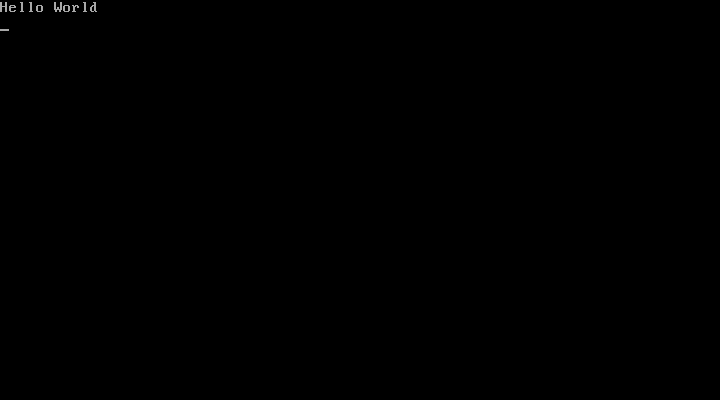
\includegraphics[width=\textwidth]{hello_world.png}
	\caption{The expected out of the current bootsector.}
\end{figure}

\section{Disk}

\subsection{Bootloading}

Great, have a working bootsector that can log messages, which is all that a bootsector really needs
to be able to do. But it is pretty obvious that we cannot fit an operating system into one 512 byte
sector. In fact, it is pretty difficult to fit a full bootloader into one single sector. A typical
bootsector's sole purpose is to load the \textit{actual} multi-sector bootloader from the disk and
jump to it. It is also pretty hard to load and parse filesystems in search of a kernel file using
just assembly too, so a typical bootsector will also make the jump to 32-bit Protected Mode before
jumping to the full bootloader which will be written in a higher level language like C.

\subsection{Loading}

Since we are still in 16-bit Real Mode, the best option we have for loading from the drive into
memory is to just ask the BIOS for us. All BIOS drive operations are under
\href{https://en.wikipedia.org/wiki/INT_13H}{interrupt \Verb|13h|}. The one we care about is
\Verb|02h|, which reads sectors from a drive.

\end{document}
